% ---------
% --------
%!TEX TS-program = pdflatex
%!TEX encoding = UTF-8 Unicode
%!TEX spellcheck = English (Aspell)

\documentclass[11pt]{article}
\usepackage{lucy,handout,graphicx}
\usepackage{fourier-orns}
\usepackage{mathtools}
\usepackage[normalem]{ulem} % either use this (simple) or
\usepackage{tikz}
\usetikzlibrary{graphs}

\allowdisplaybreaks

\begin{document}

\noindent Name \underline{\hspace{12cm}}\\


\begin{center}
\Large\textbf{CSCI 332}%
\\
\LARGE\textbf{Exam 1 Practice 1}%
\end{center}

\noindent Note that this exam has four sections. They are:

\begin{enumerate}
    \item Stable Matching (30 points)
    \item Algorithm Analysis (30 points)
    \item Graph Algorithms (30 points)
    \item Greedy Graph Algorithms (10 points)
\end{enumerate}

You may use a double sided 3x5 handwritten notecard of notes during the test but no other resources.
If you need more space than what is given, develop your solution on scratch paper before copying your final answer to the exam paper.

Good luck!

\newpage

\begin{center}
\LARGE\textbf{Section 1 (Stable Matching)\\}%
\end{center}

\begin{enumerate}
\item (5 points) The input to the \emph{stable
matching problem} is a set of $n$ men, a set of $n$ women, and preference lists
ranking each man for each woman and each woman for each man. Describe the
desired output as precisely as you can.

\vspace{1in}

\item A matching for the following preference lists for 4 men and 4 women is given by
the capitalized men and women.

\begin{center}
\begin{tabular}{ c c c }
    $m_1$: $w_3$, $W_1$, $w_2$, $w_4$ &  $w_1$: $m_4$, $m_3$, $m_2$, $M_1$\\
    $m_2$: $W_4$, $w_1$, $w_2$, $w_3$ &  $w_2$: $M_4$, $m_3$, $m_2$, $m_1$\\
    $m_3$: $w_2$, $w_1$, $W_3$, $w_4$ &  $w_3$: $m_1$, $m_2$, $m_4$, $M_3$\\ 
    $m_4$: $w_1$, $W_2$, $w_3$, $w_4$ &  $w_4$: $m_1$, $m_3$, $m_4$, $M_2$
\end{tabular}
\end{center}

    
    \item (3 points) Is this matching stable? Yes or no

    \item (2 points) How do you know?

\vspace{1in}


\item (5 points)
This is the same preference list for 4 men and 4 women given above.

\begin{center}
\begin{tabular}{ c c c }
    $m_1$: $w_3$, $w_1$, $w_2$, $w_4$ &  $w_1$: $m_4$, $m_3$, $m_2$, $m_1$\\
    $m_2$: $w_4$, $w_1$, $w_2$, $w_3$ &  $w_2$: $m_4$, $m_3$, $m_2$, $m_1$\\
    $m_3$: $w_2$, $w_1$, $w_3$, $w_4$ &  $w_3$: $m_1$, $m_2$, $m_4$, $m_3$\\ 
    $m_4$: $w_3$, $w_2$, $w_1$, $w_4$ &  $w_4$: $m_1$, $m_3$, $m_4$, $m_2$
\end{tabular}
\end{center}

 What is the outcome of the Gale-Shapley algorithm on this input? Assume that men propose to women.
\vspace{1in}

\item (5 points) True or false? In every instance of the
 Stable Matching Problem, there is a stable matching containing a pair $(m,w)$
 such that $m$ is ranked first on the preference list of $w$ and $w$ is ranked
 first on the preference list of $m$.

\newpage

\begin{center}
\LARGE\textbf{Section 2 (Algorithm Analysis)\\}%
\end{center}
\item (10 points)
For each of the following statements, circle T if it is true and F if it is false.

\begin{itemize}
    \item $2^n$ is $O(n!)$: T or F
    \item $n^3$ is $\Omega(n^2)$: T or F
    \item $n \log n$ is $\Theta(n^2)$: T or F
    \item There is an algorithm with worst-case runtime that is $\Omega(n^2)$ and best-case runtime that is $\Omega(n \log n)$: T or F
    \item There is an algorithm with worst-case runtime that is $O(n^2)$ and best-case runtime that is $\Theta(n^3)$: T or F
\end{itemize}

\item (5 points) Give a function $f(n)$ such that the worst-case runtime of the following algorithm is $\Theta(f(n))$. 

    \begin{algo}
    Algorithm-1(array $A$ of length $n$):\+\\
    Result = 0\\
    For every third $i$ in $1$ to $n$:\+\\
    For $j$ in $1$ to $i$:\+\\
    Set Result to $A[j]$ times Result\-\- \\
    Return Result\\
    \end{algo} 

    \vspace{1in}

\item (5 points) 
For the same algorithm above, give a function $g(n)$ such that the best-case
runtime of the algorithm is $\Theta(g(n))$.


\newpage

\begin{center}
\LARGE\textbf{Section 3 (Graph Algorithms)\\}%
\end{center}

\item (5 points) Finish the following algorithm to perform breadth-first search on an input graph $G$.

    \begin{algo}
    BFS(graph $G$ and starting node $v$):\+\\
    Set all nodes' layer to null, except set $v$'s to 0\\
    Set $L=0$\\
    While there is a node whose layer is null:\+\\[1in]    
    \hspace{5in}
    \end{algo} 
\vspace{1in}

\item (5 points) Give every topological ordering of the following DAG. 

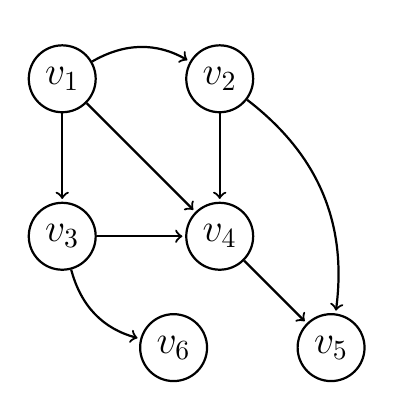
\begin{tikzpicture}[->,shorten >=1pt,auto,node distance=2cm,
                    thick,main node/.style={circle,draw,font=\sffamily\Large\bfseries}]

\node[main node] (1) {$v_1$};
\node[main node] (2) [right of=1] {$v_2$};
\node[main node] (3) [below of=1] {$v_3$};
\node[main node] (4) [below of=2] {$v_4$};
\node[main node] (5) [below right of=4] {$v_5$};
\node[main node] (6) [below right of=3] {$v_6$};

\path[every node/.style={font=\sffamily\small}]
    (1) edge [bend left] node {} (2)
        edge node {} (3)
        edge node {} (4)
    (2) edge node {} (4)
    (3) edge [bend right] node {} (6)
    (3) edge node {} (4)
    (4) edge node {} (5)
    (2) edge [bend left] node {} (5)
    ;

\end{tikzpicture}

\newpage



\item (5 points) Fill in the blanks to complete the proof that any DAG has a topological ordering.

\begin{proof}
    
Universal declaration: Let $G$ be \underline{\hspace{3in}}.

Inductive hypothesis (for this proof, use ``fewer nodes than'' for your
definition of ``smaller than''): \vspace{1in}

There are two cases to consider:
\begin{itemize}
    \item $G$ has 1 node. Then,
    \vspace{1.5in} 
    \item $G$ has $n > 1$ nodes. 
    \vspace{4in}

\end{itemize}

Since $G$ was an arbitrary DAG, and the claim holds in all cases, every DAG has a topological order.
\end{proof}

\newpage
\begin{center}
\LARGE\textbf{Section 4 (Greedy Graph Algorithms)\\}%
\end{center}


Recall Dijkstra's algorithm to compute the shortest path distance from one node $s$ to all other nodes in a directed graph with non-negative edge weights:

\begin{algo}
    Dijkstra(directed graph $G=(V, E)$ with non-negative edge weights; node $s$)\+\\
    Let $S$ be the set of explored nodes\\
    For each $u \in S$, we store a distance $d(u)$\\
    Initially $S = \{s\}$ and $d(s) = 0$\\
    While $S \neq V$:\+ \\
        Select a node $v \notin S$ with at least one edge from $S$ for which\\
        $d'(v) = \Min_{e=(u,v):u \in S} d(u) + \ell_e$ is as small as possible\\
        Add $v$ to $S$ and define $d(v) = d'(v)$\-
\end{algo}


\item (3 points) How many times \emph{exactly} does the while loop run? (This should be a function of $m$, the number of edges, and/or $n$, the number of nodes.)

\vspace{1in}

\item (3 points) Suppose that we implement the while loop naively by examining every $v \notin S$, computing $\min_{e = (u,v): u \in S} d(u) + \ell_e$, and then using those values to find the next node to add to $S$. Describe a a worst-case input for this implementation.

\vspace{2in}

\item (4 points) Assuming this naive implementation of the while loop, give a $f(n)$ such that the worst-case runtime of Dijkstra's algorithm on a graph with $n$ nodes is $\Theta(f(n))$.



\end{enumerate}

%%%%%%%%%%%%%%%%%%%%
\end{document}
